\chapter{Introduction} \label{chap1}
\noindent
As the industry attempts to maintain pace with Moore's law~\cite{moore},
design validation has become the single most complex part of the design cycle.
Today, validation accounts for more than 70\% of the design cycle time of most
chips. It is widely believed that this fraction will grow significantly in the
near future. Figure~\ref{fig1.1} shows that today's design process 
requires only 27\% of the total design effort in coding the design, the rest is 
to validate it.

\begin{figure}[htb]
\centering
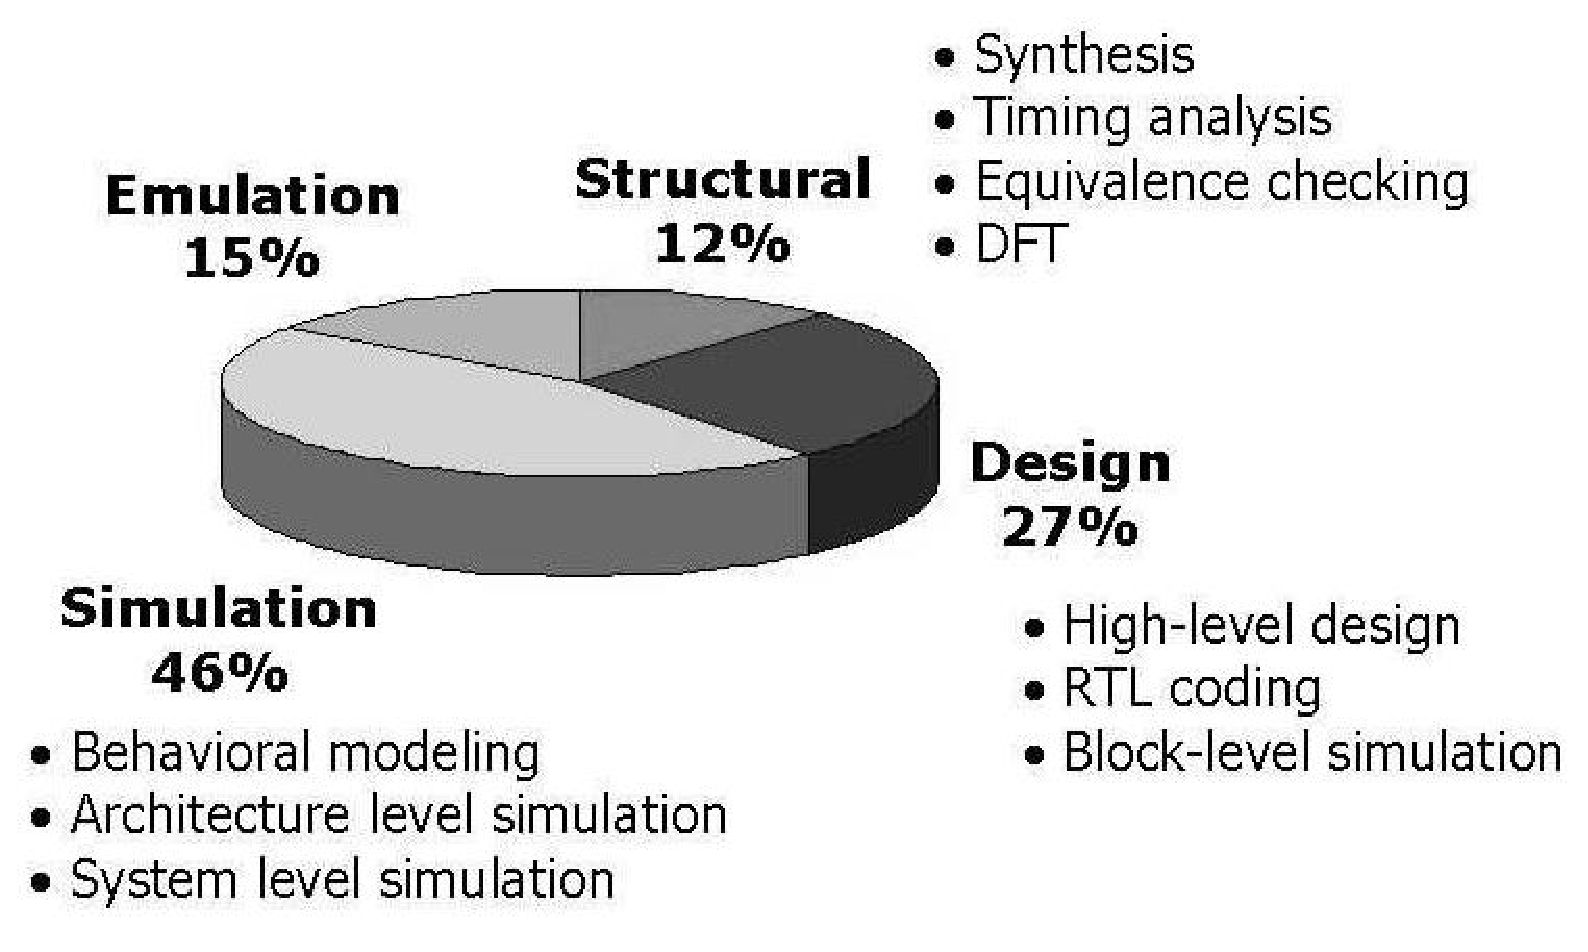
\includegraphics[scale = 0.45]{../intro/verify.eps}
\caption{Verification Dominates Design~\cite{mentor}} \label{fig1.1}
\end{figure}

\noindent
Traditional simulation based approaches to design validation proceeds by
simulating the design under test (DUT) with various test vectors that cover the
interesting behaviors of the DUT. With the growing size of designs, creating an
exhaustive set of meaningful test vectors that cover all the interesting
scenarios   has become infeasible in practice. Consequently time-to-market
constraints force the validation team to restrict themselves to a relatively
small fraction of the interesting behaviors. The main challenge today is to
achieve greater coverage in less time. 

\noindent
In recent times, most leading companies are seriously investigating the possibility of
integrating property verification into their validation flows.
Property verification is predominantly used in two forms in 
validation, namely (a) Dynamic Property Verification (DPV), and
(b) static Formal Property Verification (FPV). In both forms, the properties
are written in a formal specification language. DPV is a simulation-based
approach, where the properties are checked over a simulation run -- the
verification is thereby confined to only those behaviors that are encountered
during simulation. FPV techniques formally verify whether {\em all} possible
behaviors of the design satisfy the given properties. The promise of
exhaustive validation is one of the main attractions of FPV technology. It is
unrealistic to obtain a similar guarantee through simulation driven approaches,
in view of the number of intricate directed tests that would be required to
achieve full coverage of potential behaviors. Unfortunately, FPV technology
today does not scale beyond small circuit modules, due to its requirement
of huge computing resources. DPV, however, being simulation-based, is scalable.
This {\em verification crisis} has inspired a recent trend
towards the deployment of semi-formal techniques which combine both
formal search and simulation-based techniques in a unified setting,
thereby, attempting to provide a scalable and more comprehensive
validation solution. 

\noindent
Developing a formal specification that correctly and completely captures the
design intent is a non trivial task. At the same time, well-designed 
formal specifications play a crucial role in expediting the performance 
of property verification technologies. The focus of this research is in 
proposing new formal methods for accelerating formal, semi-formal and 
dynamic property verification through some novel specification styles. We 
believe that the methods arising out of our research 
will lead to wider adoption of property verification in the
validation flow of ASL.

\begin{figure}[htb]
\centering
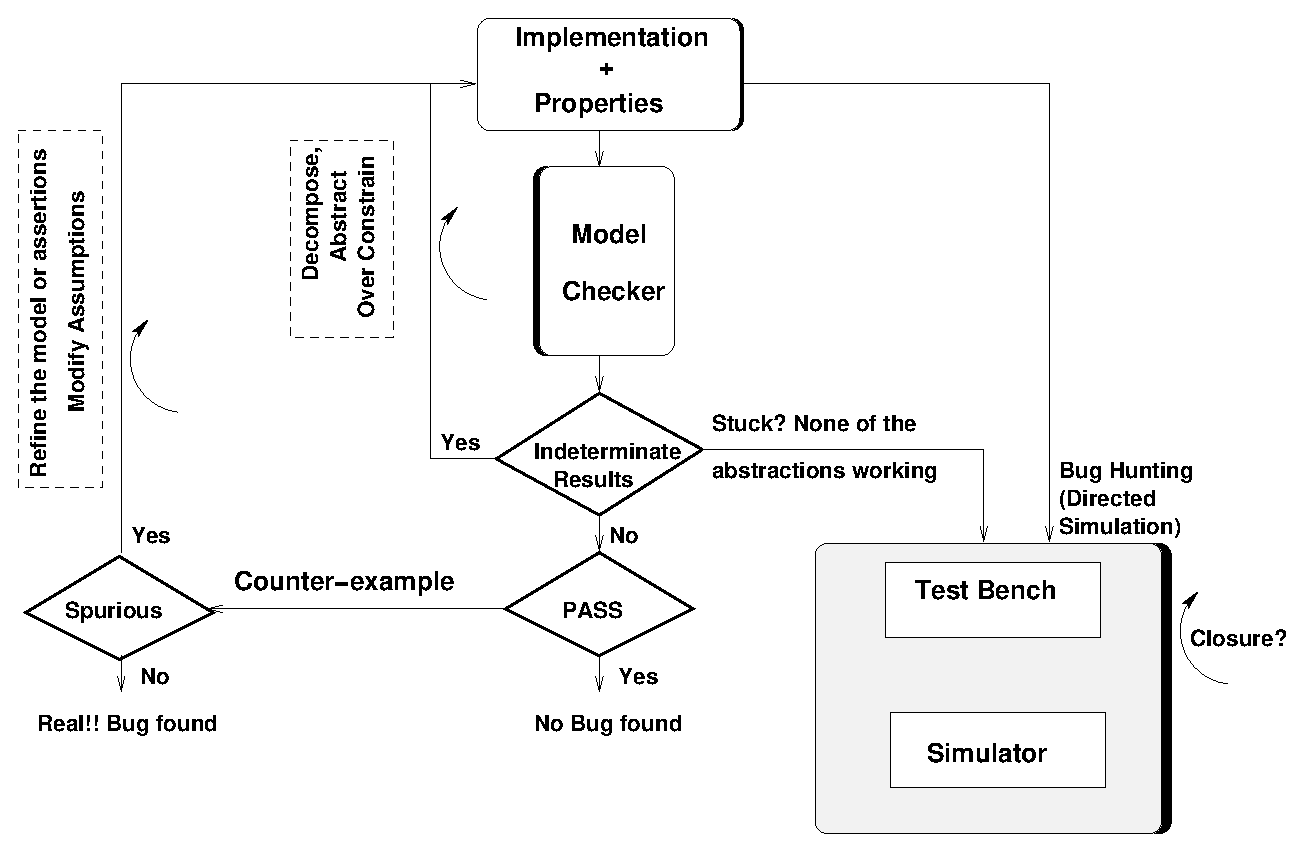
\includegraphics[scale = 0.7]{../intro/intro.eps}
\caption{Emerging Validation Flow} \label{fig1.2}
\end{figure}

\section{Emerging Validation Flow} \label{sec1.1}
Figure~\ref{fig1.2} shows the property verification flow employed today 
in most leading chip design companies. Typically companies prefer to use 
FPV before simulation. At the heart of this approach we have a 
{\em model checking} tool. A model checking algorithm has two main
inputs -- a formal property in a property specification language 
(e.g. Linear Temporal Logic (LTL)~\cite{pnueli:77}, Computation Tree Logic 
(CTL)~\cite{clarke:86}, System Verilog Assertions (SVA)~\cite{sva}, 
Property Specification Language (PSL)~\cite{psl}, ForSpec~\cite{forspec}) 
and a finite state machine representing the
implementation. The role of the algorithm is to search all possible paths
of the state machine for a path which refutes one or more properties. If one
exists, then the path trace is reported as the counter-example. Otherwise
the model checker asserts that the property holds on the implementation.

\noindent
The main bottleneck of FPV is in its space complexity. If we can fit the
state machine of the implementation in memory, then FPV works well. Otherwise
it runs into capacity issues.
This limitation has encouraged many researchers to study the task of creating
abstractions of the implementation. Some abstractions preserve the truth of
properties in given languages. For example bisimulation 
equivalence~\cite{clarke:00} abstractions preserve most temporal languages, 
and stuttering equivalence~\cite{clarke:00} abstractions preserve untimed 
temporal logics without the $X$ operator. These
abstractions are {\em safe} -- if our property fails on the abstraction, then
it is guaranteed to fail in the implementation, and vice versa. 

\noindent
Safe abstractions do not always give us the desired reduction in space -- they
are often too big. It is possible to create much smaller abstractions, but
they may not preserve the truth of all the properties in the specification.
In such cases, two things may happen:
\begin{enumerate}

\item A property evaluates to true in the abstract model, but is actually
    false in the implementation. This means that a bug escapes detection,
    and this defeats the whole purpose of {\em formal} property
    verification.

\item A property evaluates to false in the abstract model, but is actually
    true in the implementation. This means that our abstract model
    produces false counter-examples -- ones that do not actually exist
    in the implementation.

\end{enumerate} 
\noindent
The first is obviously the worse among the two. Therefore, abstractions are
made in such a way that the first never happens. In other words, if the
abstract model satisfies the specification, then the implementation is
guaranteed to satisfy the specification.

\noindent
To verify the soundness of a counter-example, a common approach is to use
simulation. We want to verify whether the counter-example
trace produced by the model checker from the abstract model is real or 
spurious, that is,
whether we can reproduce the counter-example in the implementation. We perform
this test by simulating the implementation using the valuations of the input
signals in the counter-example trace. If the simulation reproduces the
counter-example, then we have indeed found a bug. 
In case it is not, the model and/or the assertions 
are refined and the process is repeated.
This method is popularly known as {\em counter-example guided abstraction 
refinement}~\cite{clarke:00b}.

\noindent
It is not always easy to generate safe abstractions that are of manageable 
size. This is therefore, an iterative process, as shown in 
Figure~\ref{fig1.2}. The process is repeated till the size of the abstract 
model is within capacity limits of the model checking tool. Several 
abstraction mechanisms (to be discussed in Chapter~\ref{chap2}) have 
been proposed in literature. In the worst case, none of the abstractions 
of the implementation can be handled by the model checking tool. In such 
a case, the validation methodology switches to a simulation-based bug 
hunting mode. 

\noindent
In the bug hunting mode, the set of assertions and the original 
implementation are simulated by a test-bench. 
Validation engineers identify the set of interesting 
behaviors where they believe bugs may hide. A test plan is developed to 
cover the set of interesting behaviors. The test plan consists of a set 
of tests that together achieve the desired level of coverage. 
Directed tests are written for each item of the test plan. For each test,
the validation engineer has to write a test bench to mimic the
environment of the design-under-test (DUT) and drive the appropriate
stimuli to reach the desired coverage points. Simulation is performed for 
each of the directed tests, and success/violation of the assertions are 
reported.

\subsection{Challenges in the Emerging Validation Flow} \label{sec1.1.1}
The capacity limitation of existing FPV tools is at the heart of the 
problem, which necessitates creating smaller modules or abstractions 
of the design implementation that can be handled. Creating a safe 
truth-preserving abstraction of a design is a non-trivial task. 
This decomposition/abstraction step requires an in-depth understanding of 
the design and specification and involves a lot of additional tasks. 
Moreover, the design decomposition has to be accompanied by a 
decomposition in the specification -- to generate module-level specifications 
and constraints from the system level specification. This is probably, the 
biggest challenge associated with the design decomposition step, since 
existing temporal logics do not easily lend themselves to automatic 
decomposition of system-level specifications. In particular, 
module-level specifications end up in a lot of semantic anomalies that 
perplex the validation engineer, and lead to wastage of validation effort. 

\noindent
Arriving at the right set of assumptions in the design refinement loop 
is another important challenge of the flow shown in Figure~\ref{fig1.2}. 
These assumptions have to be really effective in improving the scalability 
of the model checking tool. In particular, these {\em assume constraints} 
are used to prune the state machine of the implementation, since we need 
not consider those runs of the implementation that violate the assume 
constraints. In many cases, this can lead to significant reduction in 
the size of the reduced state machine. 

\noindent
Achieving closure in the bug hunting loop is one of the toughest 
challenges in the emerging validation flow in Figure~\ref{fig1.2}.
As the design complexity increases, we face two problems, namely (a) the
number of directed tests required to cover all the interesting behaviors
grows alarmingly, and (b) the task of writing each directed test becomes
more complex, thereby requiring more time from the validation engineer. 

\noindent
As the complexity of the design grows, the number of properties required to
express the design intent grows, and with it grows the possibility of 
inconsistencies in coding assertions. 
If designers can make mistakes while writing 
the code, they can make mistakes while writing assertions as well. 
Beyond a point, human debugging of the 
specification becomes infeasible because many properties may together 
create a conflict. 
Inconsistent specifications lead to the loss of validation
productivity, since the error lies in the specification itself.
This is one of the main challenges faced by every chip design company that
uses static or dynamic property verification in its validation flow. In
these early stages of adoption of property verification, the problem is more
glaring. This is because a company will have many designers
who understand coding, but relatively few who understand an assertion
language. Debugging code has been cultivated for decades. Debugging
a set of assertions is new and not fully understood by most.

\section{Motivation of this research}
The main aim of this research is to study the role of formal specifications 
in addressing the challenges identified above in the property verification 
flow in the context of the ASL systems. 
Interestingly, most of the formal specification research has focused mainly on 
developing property verification tools or inventing languages. For tools, 
much effort has gone into improving the horsepower of these tools to 
make them more widely usable. A plethora of specification languages for 
expressing property requirements have been introduced. In this context, it 
is important to note that the objective of this research is {\em not to} 
propose a new specification language or verification paradigm for software
development, but rather to formalize a set of verification styles 
that can be applied to any existing language. This language independence 
allows our specification styles to be applied to any software code, 
and give better verification performance, while retaining the 
existing capabilities of such languages. As a concrete research 
objective, we will investigate specification styles that facilitate 
abstractions in the context of software and hardware-software systems, 
with specific applications to the ASL designs.

\subsection {Specification paradigms}
Formal specification techniques typically differ by the particular 
specification paradigm they rely on. In the sequel, we mention a few 
of the popular specification development paradigms. 

\begin{description}

\item [History-based Specification:] The principle here is to specify 
	a system requirements by characterizing its maximal set of 
	admissible histories. The properties of interest are specified 
	by temporal logic assertions about system objects; such assertions 
	involve operators referring to the past, current and future states. 
	The assertions are interpreted over time structures. Time can 
	be linear (LTL) or branching (CTL). Many of the temporal logics 
	support the ability to express history using a {\em past} 
	operator.

\item [State-based Specification:] Instead of characterizing the set 
	of admissible histories, one may characterize the admissible system 
	states at some arbitrary snapshot. The properties of interest are 
	(a) invariants constraining the system objects at any snapshot, and 
	(b) pre- and post-assertions constraining the application of 
	system operations at any snapshot. Examples of this specification 
	style can be found in~\cite{Abr80, Abr96}.

\item [Transition-based Specification:] Instead of characterizing 
	system histories or states, one may characterize the required 
	transitions from state to state. The properties of interest are 
	specified by a set of transition functions; the transition 
	function specifies for each input state and triggering condition, 
	the set of allowable behaviors. Languages such as Statecharts, 
	PROMELA or SCR rely on this paradigm.

\item [Functional Specification:] The principle here is to specify the 
	system requirements through a collection of mathematical functions. 
	Languages such as OBJ~\cite{fut95}, HOL~\cite{gor93} or 
	PVS~\cite{cro95} rely on this paradigm.

\item [Operational Specification:] System properties may be characterized by 
	a collection of processes that can be executed by some more or 
	less abstract machine. Early languages such as Paisley~\cite{zav82}, 
	Petri Nets rely on this paradigm.

\end{description}

\noindent
In addition to the ones mentioned above, there exist many more 
specification paradigms that have been used by the verification 
community. Different specification paradigms can have different effects on 
different property verification techniques, in terms of power of 
expressibility and verification performance. This was one of the motivations 
of this research.

%\subsection{Objective of this research}
\noindent
The main motivation of this research is to address some of the challenges 
of the emerging validation flow as identified in Subsection~\ref{sec1.1.1}. 
In particular, this research has two main motivations:

\begin{itemize}

\item We believe that the scalability and efficiency of formal and
    semi-formal verification can be improved by adopting specification styles
    that syntactically facilitate abstractions and pruning in the context 
    of hardware-software systems.

\item We believe that assertion coverage by constrained random 
    simulation can be improved by guiding the simulation through formal
    methods.
\end{itemize}

\noindent
The main aim of this research is to study the above issues
and propose methods for accelerating formal, semi-formal and dynamic
property verification in the context of hardware-software systems. 
In particular, we wish to achieve some of the following objectives 
in the years to come.

\begin{description}

%\item [Accelerating assertion coverage in DPV:] 
%	The success of verification depends largely on the coverage of the 
%	scenarios that are relevant to the properties that constitute the 
%	property suite. The mere existence of a property that guards against a 
%	given bug is not enough to detect the bug unless the simulation of 
%	the design-under-test (DUT) covers all input scenarios that may 
%	trigger the faulty behavior. This inspired us to develop automated 
%	techniques that can analyze formal specifications and spin off 
%	the tests that are required to trigger them during simulation.

\item [Improving the specification style for verification:] 
	Formal specifications should have 
	adequate expressibility and lend themselves easily to express 
	functional requirements. For certain classes of functional 
	requirements, the choice of the specification style is crucial, 
	since a wrong selection will force the specification developer to 
	write unnecessarily complicated properties. An important observation 
	in this context is that some assertions are typically written for 
	specific scenarios -- in other scenarios they are satisfied {\em vacuously}.
	This information can be utilized to make the verification process 
	more effective, both in terms of FPV and bug hunting. 

\item [Improving FPV scalability:] Existing model checking tools can
	only handle code blocks of small size. These are typically open
	systems, that is, their behavior is a function of the inputs that
	they receive from the other components of the design. In order to
	verify the block in the context of the design, we need to model the
	behavior of the neighboring components as well, so that the
	verification considers only meaningful inputs into the block. 
	This will need research on new specification styles that can allow 
	one to model the appropriate assumptions on the input behavior of a
	block along with the correctness requirements, and to verify the 
	functionality of the block under these
	assumptions. We attempt to overcome the capacity issue by 
	verifying each block separately -- each block is verified under
	appropriate assumptions on the remaining blocks.

\item [Consistency Analysis:] Consistency analysis is of immense 
	importance in the specification development life cycle, and requires 
	good support, both in terms of efficiency of algorithm and tool support. 
	Unfortunately, the complexities of the consistency analysis procedures 
	for temporal logics like Computation Tree Logic (CTL) and Linear Temporal 
	Logic (LTL) are very high. This may need us 
	to adopt subsets of existing temporal logics with lesser expressibility 
	and lower consistency checking complexity. 
	
\item [Property verification for hardware-software systems:]
	We wish to investigate the role of property verification 
	in the context of software systems and more generically, hardware-software 
	systems.
	Correctness requirements arising in software are somewhat different 
	from those in hardware, and thereby require additional constructs in 
	temporal logics. This may need us to extend existing temporal logics, 
	in particular, LTL, with additional features for expressing correctness 
	requirements arising in software. In addition, we may need to develop a complete 
	solution for validating such properties over hardware-software / firmware.
\end{description}

\begin{comment}
\noindent
The above objectives led to new specification styles that necessitated new 
verification methods. The main contributions of this thesis are highlighted in 
the following section.

\section{Contributions of this dissertation} \label{sec3}
The focus of this thesis was to examine the role of formal specifications in 
the different facets of property verification and come up with an arsenal 
of novel specification styles that can facilitate larger penetration of 
property verification into the validation flows of companies. 
In particular, this thesis proposes new formal methods 
for accelerating formal, semi-formal and dynamic property verification 
through novel specification styles.
The following subsections highlight the contributions of this thesis.

\subsection {Accelerating Assertion Coverage using Adaptive Test Benches}
\noindent
The main lacuna of DPV, that is, checking assertions over simulation
runs, is that the verification is not exhaustive. FPV verifies a
given property over all possible traces of the design-under-test (DUT),
where as DPV verifies the property over only those traces that are
covered by simulation. FPV may hit a bug that refutes some assertion,
where as the bug may be missed by DPV because the simulation did not
cover any of the counter-example traces for that assertion. 

\noindent
The success of a DPV property suite
depends largely on the simulation coverage of the scenarios that
are relevant to the assertions that constitute the property suite.
The mere existence of a property that guards against a given bug is not enough
to detect the bug unless the simulation of the design-under-test (DUT)
covers all input scenarios that may trigger the faulty behavior.
An important observation in this context is that an assertion is typically
written for a specific scenario -- in other scenarios it is satisfied
{\em vacuously}. For example, consider the following property for a
typical Bus protocol:

"In a burst mode transfer, addresses wrap around the 2kb address boundaries"

\noindent
It is easy to see that the property is relevant only during burst
mode transfers. The test-bench must drive burst-transfers if we are
to check this property.

\noindent
In DPV parlance, an assertion is said to be {\em covered} each time
the simulation hits a scenario where it is checked non-vacuously.
The definition of {\em vacuity} is not uniform, and verification
engineers use various metrics for assertion coverage. In many tools, 
an assertion in implication form is said to be covered whenever the
antecedent part of the implication matches. For example, consider
the following property for an arbiter with input $r$ and 
output $g$ which says that {\em if the request $r$ is asserted then
the grant $g$ must be asserted in the next two cycles, unless $r$
is lowered in between}:
{\tt
\begin{tabbing}
a \= aaa \= aaa \= aaa \= aaa \= \kill
\>\>\>{\cal P}: G (r $\Rightarrow$ X (g $\lor$ ($\neg$ g $\land$ $\neg$ r)
$\lor$ ($\neg$ g $\land$ r $\land$ X g)))
\end{tabbing}}

\noindent
Obviously, the above assertion is vacuously satisfied in all traces
where $r$ is never asserted. Some tools will report the assertion
to be covered each time $r$ is asserted, because $r$ satisfies the
antecedent of the implication. This is not really a formal
definition of vacuity, since we could write the same property
without using the implication operator -- in which case the context
of the property would become implicit. 

\noindent
Implication vacuity also overlooks a very important fact which is
demonstrated by the scenario when the test-bench drives $r$ at
cycle $t$ but does not get the grant $g$ in the next cycle, $t+1$.
In this case, the test bench must drive $r$ again to test whether
the arbiter asserts $g$ at $t+2$, because if it doesn't, then $P$
will be refuted. On the other hand, if the test bench lowers $r$
at $t+1$, then the property will be satisfied vacuously. In other
words, the coverage of a temporal property (like $P$) may continue
over many cycles and we have a coverage hit only when the response
of the design-under-test eventually decides the truth of the
property.

\noindent
Driving a non-vacuous scenario is therefore a game between the DUT
and its test bench. In each cycle (round of the game), the test
bench must choose the values of the inputs to the DUT in a way
such that the truth of the assertion is not solely determined by
the values of the input signals, but depends on the response of the
DUT in the next cycle. The property is satisfied non-vacuously if
the response of the DUT eventually decides the truth of the
assertion. Chapter~\ref{chap3} presents this concept in greater detail.

\noindent
Designs often have correctness requirements under corner case scenarios that
occur rarely, but are of considerable significance from the point of view of
functional correctness. Experience shows that random test generators often
fail to create these corner case scenarios in reasonable time because the
probability of such scenarios is low.
As a result, the validation engineer manually writes directed tests to create
corner case scenarios to cover the behaviors targeted by the complex
temporal assertions. It is not easy to determine the complex input sequences
that trigger an assertion by visual examination. Therefore, 
one of the main challenges in the current DPV framework is to develop formal 
methods for automatic test generation from temporal assertions. This is 
one of the contributions of this work.

\noindent
Another contribution of this work is to generate a test bench that is  
intelligent and adaptive -- in the sense that, it should
be able to diagnose imminent failures during simulation
when the DUT makes a mistake and
guide the simulation to expose an assertion refutation as well. This
is typically the case, when we have unreceptive specifications
in our coverage goal. 
Unreceptive specifications may create a debugging problem in dynamic property
verification. The reason is as
follows. With unreceptive specifications, the failure of a property may take
place several cycles after the sensitization of a fault in the DUT. Worse
still, a fault may get masked before it is detected unless proper inputs are
driven by the test bench. In other words, the fault can be propagated
through the cycles by an intelligent choice of inputs until it refutes a
property. We elaborate more on these formal methods in Chapter~\ref{chap3}.

\noindent
In all forms of test generation games, we must realize that the test bench has
to drive many other signals that do not appear in a given assertion.
In other words, while targeting a given assertion, the test bench must
drive the other signals also in a compliant manner -- a task
which is hard to automate. A more practical approach would be to embed
our formal methods within an existing test bench architecture, so that
the test bench queries our formal method in each cycle for
the values of only those inputs that are relevant to the target assertion.
We have taken this approach to integrate our methods with layered
constrained random SystemVerilog~\cite{sva} test bench architectures and have
achieved considerable success in terms of a dramatic improvement 
in assertion coverage.

\subsection {Context-Sensitive Specifications} 
An analytic study of the formal specifications for a
multitude of protocols (e.g. ARM AMBA~\cite{ahb}, IBM 
CoreConnect~\cite{ibmcc}) has led us to believe that formal specifications of
interface protocols mostly consist of two types of
correctness requirements, namely (a) a set of invariants
that applies throughout the protocol execution and (b) a set of
{\em context-sensitive} properties that applies only when the protocol is in a
specific set of contexts (bus acquisition context, transfer context etc.)
For example,
the mutual exclusion property for an arbiter (which specifies that
the arbiter issues one grant at a time) is an invariant property,
whereas a property which specifies that successive addresses must
wrap around 2KB address boundaries may be applicable only in the
context of burst transfers (and not in general). For properties
of the second type, we need to model the context, which is not
easy in terms of formal property languages since in many cases,
the context cannot be defined in terms of the current signal
values and depends on the history of the protocol. In our
experience, context-sensitive properties account for a large
percentage of the properties in complex protocols. 

\noindent
In order to facilitate the development of context-sensitive
properties, researchers~\cite{pdgbook,dill:01} have
suggested the use of {\em auxiliary state machines} to model the abstract
states of the protocol. These state machines become part of the formal
specification and significantly ease the development of
context-sensitive properties, which can now use the states
of the auxiliary state machines to define the context of the
property. The auxiliary state machines typically contain a
small subset of the DUT interface signals, whose valuations are
needed to characterize the major protocol contexts and the
context switches. This keeps them small and simple. 
We explain the advantages of this style of
specification with the following example.

\begin{figure}[htb]
\psfrag{start} {\tt \bf start}
\psfrag{!req} {\tt \bf $\neg$ req}
\psfrag{req} {\tt \bf req}
\psfrag{!rdy} {\tt \bf $\neg$ rdy}
\psfrag{rdy} {\tt \bf rdy}
\psfrag{reqgnt} {\tt \bf req $\land$ gnt}
\psfrag{reqngnt} {\tt \bf req $\land$ $\neg$ gnt}
\centering
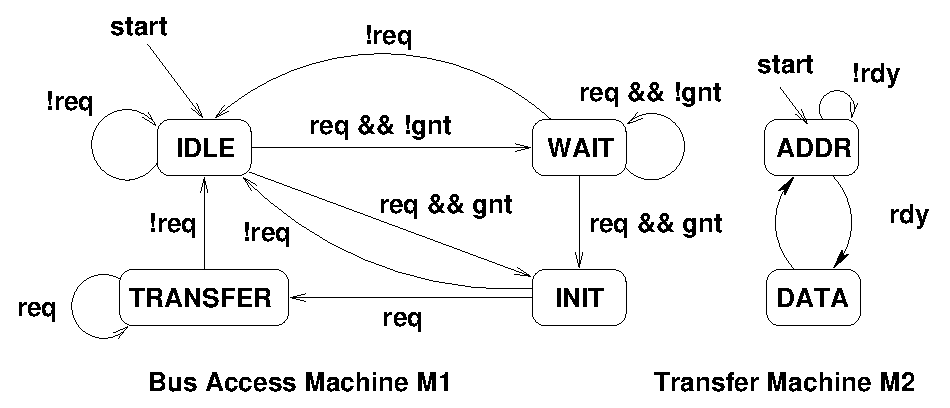
\includegraphics[scale=0.9]{../tcad07/diag217.eps}
\caption{Auxiliary State Machines} \label{fig1.3}
\end{figure} 

\begin{example} \label{example1.1}
{\em 
Consider the specification of a master interface participating in a simple bus
protocol with an arbiter and a slave device. Fig~\ref{fig1.3} shows two
auxiliary
state machines for describing the macro states of the protocol. $M1$ describes
the state of the master during bus access in terms of {\tt req} (request to
arbiter) and {\tt gnt} (grant from arbiter). $M2$ describes a more detailed
state
of the master during the transfer using the signal {\tt rdy} (slave ready). 
Note that the auxiliary state machines involve a small fragment of the 
DUT interface
signals. For our master interface, there are other signals, namely,
(a) {\tt rw} (indicating the nature of current transfer, write or a read),
(b) {\tt validaddr} (flag indicating the validity of the address 
floated on the bus)
(c) {\tt abort} (transfer terminated by the slave), and
(d) {\tt delayed} (delayed transfer).

\noindent
The specification of the master (DUT) includes the following properties:
\begin{itemize} 
\item ${\cal P}_0$: If the transfer waits due to non-availability of slave
        while
        the abort signal is low, then the delayed signal should be asserted
        in the next cycle.

\item ${\cal P}_1$: If the master is in the ADDRESS cycle in a write transfer,
        it should always hold a valid address in the next cycle.

\end{itemize}

\noindent
Both properties are context-sensitive. ${\cal P}_0$ applies only when the 
master is in the waiting phase, whereas ${\cal P}_1$ applies only when the 
master is in
the ADDRESS phase. It is easy to code these properties using the auxiliary
state machines, as shown below.
{\tt
\begin{tabbing}
aaaa \= aaa \= aaaaaaaa \= aaaa\= aaaaa\= \kill 
\>\>\> ${\cal P}_0:$G(WAIT $\land \neg$ abort $\Rightarrow$ X\ delayed) \\
\>\>\> ${\cal P}_1:$G(TRANSFER $\land$ ADDR $\land$ rw $\Rightarrow$ X validaddr)
\end{tabbing}
}

\noindent
Though specifications consisting of auxiliary state machines and
context-sensitive properties can alternatively be expressed purely in terms
of temporal logic properties, such representations become quite
unreadable in practice. The auxiliary state machine defines a labeling
of the states of the DUT by the different contexts, and characterizing the
set of states labeled by a specific context through a temporal logic
expression is not convenient. For example, the context {\tt INIT} can be
reached from the {\tt IDLE} context in many ways (either directly or via the
{\tt WAIT} context, or possibly stuttering at the {\tt WAIT} context
for an arbitrary number of cycles). 

\noindent
Context-sensitive properties, therefore, have a clear advantage in
expressing the desired intent, since the context can be specified
succinctly by referring to states of the auxiliary state machines. 
}
$\Box$
\end{example}

\noindent
It is important to note that auxiliary state machines are developed
independently by the verification engineer as an integral part of the
formal specification -- they are not part of any given implementation,
nor are they extracted out of one. Also protocol specs often provide
such abstract state machines (for example, the ARM AMBA protocol
specs).

\noindent
Chapter~\ref{chap5} presents the formal model for this style of formal 
specifications consisting of auxiliary state machines and context-sensitive 
properties.

\subsubsection{Verifying Context-Sensitive Properties}
We now consider the task of verifying context-sensitive properties on a 
given DUT. Ideally, we wish to verify a context sensitive property $\varphi$ 
from the DUT states that satisfy the context of $\varphi$. Therefore, we need 
a methodology to identify the context-satisfying DUT states. For example, to 
verify ${\cal P}_0$, we need to first reach DUT states that model the 
$WAIT$ context. 

\noindent
In our work, we consider two different approaches for this task, namely:
\begin{enumerate}

\item Use of simulation to drive the DUT to a context-satisfying state, and
    verifying the properties formally from that state.

\item Use of a formal approach for extracting all DUT states that
    are labeled by a given context and verifying the properties
    formally from that set of states.

\end{enumerate}

\noindent
The two approaches differ in terms of the method used to reach the
states labeled by a given context. In the first approach which is a
semi-formal one, we reach the context-labeled states through simulation.
In the latter, we formally extract all the states labeled by a given
context. In both approaches, we use a BMC-based formal
search to verify the context-sensitive properties from the
context-labeled states. In the semi-formal approach, we may not reach
all reachable states receiving a given context label, whereas in the formal 
approach, we exhaustively cover each of these states.
Below, we briefly explain each of these approaches.

\subsubsection{Semi-Formal Verification with context-sensitive properties}
\noindent
The semi-formal approach adopted by us combines simulation 
and BMC in an attempt to localize the formal search from the 
context-satisfying states. It may be noted here that a purely random simulation 
approach is not the right choice for driving the DUT to a 
context-satisfying state, since the chance of hitting the target context 
depends on the random test generator for providing the required inputs. 
Therefore, to make this task more effective, we use a constrained random 
approach, as explained below. The approach adopted by us consists of two steps:
\begin{enumerate}
\item In the first step, we use the auxiliary state machines to generate 
	inputs that can bias the simulation test generator to generate 
	context-guiding inputs that can drive the DUT to a state satisfying the 
	target context. %We treat the DUT as a black-box and generate 
	%inputs by analyzing the context-switching transitions in the auxiliary 
	%state machines. Since the auxiliary state
    %machines contain both input and output signals of the DUT, this
    %step is a game between the DUT and the test-bench, where the
    %test-bench wins if a context-satisfying state is reached.
\item Once a context-satisfying state is reached, we use BMC to verify
    the context sensitive property from that state.

\end{enumerate}

\noindent
The proposed
methodology was integrated with two popular verifiers, namely, 
Magellan~\cite{magellan} and VIS~\cite{vis} with dramatic
improvement in performance -- in terms of speed and scalability. 
Chapter~\ref{chap5} presents this approach in greater details. 

\subsubsection {Formal Verification with Context-Sensitive Specifications}
The use of simulation 
to guide the DUT to context-satisfying states limits our approach to only the 
DUT behaviors explored during simulation, and hence, we end up tracing 
a single path from the DUT start state to a single context-satisfying state 
in the implementation. We need to rerun the semi-formal engine multiple 
number of times with adequate measures to be able to explore other paths 
to other context-satisfying states in the DUT implementation. 

\noindent
This motivated us to look for a formal approach for identifying 
the DUT states that satisfy a given context.
The main objective of our approach is to 
verify context-sensitive properties from {\em all} DUT states that 
satisfy the context. This achieves exhaustive coverage in terms of DUT 
behaviors examined with respect to the context of 
a context-sensitive property. In Chapter~\ref{chap4}, we adopt a 
subset of context-sensitive properties and explain our 
methodology. 

\noindent
Our approach has two main steps:
\begin{enumerate}
\item In the first step, we formally extract all DUT states that
    are labeled by a given context.
\item In the second step, after all context-satisfying DUT states 
	are identified, we use a BMC-based formal search to verify the 
	property with these states as initial states.
\end{enumerate}

\noindent
Chapter~\ref{chap4} explains the above steps in greater detail.
We integrated our methodology on top of VIS~\cite{vis}. Results 
show an improvement in memory requirement.

\subsubsection {Realizability of Context-Sensitive GR (1) LTL}
The problem of checking realizability of temporal logic specifications
has been one of the most challenging problems before the validation
community for decades and has been an area of active 
research~\cite{ce81,mw84,pnueli:89,prosyd}.
The high complexity of the LTL realizability problem (LTL realizability is 
2-EXPTIME complete~\cite{pnueli:89}) and the intricacy of
the determinization construction involved in solving the realizability
problem inspired considerable research in finding fragments of LTL
for which the realizability checking complexity is lower~\cite{alur:04}.
In~\cite{nir}, Peterman
et al. have identified a fragment of LTL, known as Generalized
Reactivity (1) (GR (1)), for which the realizability problem can be
solved in EXPTIME. This is a significant improvement.

\noindent
The motivation behind our work in Chapter~\ref{chap6} is to investigate the
complexity of the realizability problem for the language consisting of
formal specifications with auxiliary state machines
and context-sensitive properties in GR (1) LTL.
As a positive result, we show in Chapter~\ref{chap6}, that this mixed 
specification
language (auxiliary state machines + context-sensitive GR(1) LTL) can be
reduced to GR (1) LTL without any additional blowup in the
length of the property, and therefore, has a lower realizability checking
complexity. With the increasing adoption of this mixed modeling
style in designing verification IPs, we believe that our analysis is
of significant importance to the validation community. 

\subsection {Annotating Temporal Operators with Input Constraints}
In view of the inherent capacity limitation of FPV techniques, there has 
been a paradigm shift from a system level validation perspective to a 
modular validation one. A design typically consists of a set of interacting 
modules. The validation
task in this new perspective amounts to verifying each module in
isolation (module checking) and then verifying their interaction protocols.

\noindent
A module is an open system which interacts with its environment
and whose behavior depends on this interaction. The environment of a module
consists of the responses of its peer modules with which it interacts through
its interface. Validating the module against all possible valid environments
is again an explosive task. In reality, only a subset of the possible
environments needs to be modeled on the basis of the environment interactions
which can affect the module behavior. The main challenge in modular 
verification lies in modeling this interaction. 
Researchers have studied a few approaches for modeling the 
module-environment interaction. One approach defines 
an interface
process (an interface of a module consists of its input-output behavior)
and verifies a module in isolation by composing the module
behavior with its interface. The interface process mimics the behavior of the
environment of the module and thus the desired verification task is
accomplished. In a second approach, for each module, the original
specification is partitioned into the assume and the guarantee
and the module is checked to determine whether it satisfies the guarantee
in presence of the assumptions, and a composition rule is defined to compose
the verification tasks for each module to reason about the entire system.
However, both the above approaches are non-trivial. The
construction of the interface process is difficult in the former approach while
the latter approach is non-trivial due to the inherent intricacy involved
in assume-guarantee separation of the specification.

\noindent
In our work, we have proposed a new style for modeling this interaction. 
Our motivation was the fact that formal property 
specification languages like Computation Tree Logic (CTL) or Linear Temporal 
Logic (LTL) were originally developed for closed systems. These languages, 
therefore, do not lend themselves
easily to the specification of behaviors of open systems, and thereby, 
give rise to several semantic problems. We elaborate on these in 
Chapter~\ref{chap7}. 

\noindent
To address these inadequacies, we have proposed an extension of 
Linear Temporal Logic (LTL), called Open Linear Temporal Logic (Open-LTL).
The fundamental change introduced in Open-LTL allows the basic
temporal operators to be associated with environment constraints.
The novelty of this logic is that it integrates the specification of the
property to be verified with the
valid input patterns under which it is expected to hold. For example, while
the LTL property $Fq$ asks whether $q$ holds sometime in the future, the
Open-LTL property $F_{\cal I}q$ asks whether $q$ holds sometime in the
future provided the environment continues to assert the input ${\cal I}$.
Intuitively, the input annotation ${\cal I}$ specifies exactly those
environments under which the property $q$ is to be verified. Open-LTL
is our proposed extension of LTL, which allows annotations of the basic
temporal operators {\em next} and {\em until} with input assumptions.
Open-LTL is very useful for expressing properties of modules, since
they allow the specification of properties and input constraints in a unified
way. 

\noindent
To illustrate the power of our proposed logic,
we now present a simple example of how Open-LTL helps in making
queries that incorporate knowledge about the environment. Knowledge about
the environment can be gleaned from the descriptions of the individual
peer modules or from the peculiarities of the system designed. We consider 
a simple PCI-compliant system consisting of a single master and a single 
target device. Figure~\ref{fig1.4} shows the state transition
system for an abstract model of a PCI target (slave) device. 
The environment of the target device consists of the master device.

\begin{figure}[htbp]
\psfrag{TBUS}{\small \bf \tt busy}
\psfrag{NTBUS}{\small \bf \tt $\neg \mbox{busy}$}
\psfrag{FRAME}{\small \bf \tt frame}
\psfrag{NFRAME}{\small \bf \tt $\neg \mbox{frame}$}
\psfrag{NFRAMENADDR}{\small \bf \tt $\neg (\mbox{frame} \land \mbox{address})$}
\psfrag{FRAMETBUS}{\small \bf \tt $\mbox{frame} \land \mbox{busy}$}
\psfrag{FRAMENTBUS}{\small \bf \tt $\qquad \mbox{frame} \land \neg \mbox{busy}$}
\psfrag{FRAMEADDRAND}{\small \bf \tt $\mbox{frame} \land \mbox{address} \land$}
\psfrag{TBUSRESP}{\small \bf \tt $\mbox{busy} \land \mbox{respond}$}
\psfrag{NRESP}{\small \bf \tt $\neg \mbox{respond}$}
% \psfrag{FRAMEADDRTBUS}{\small \sc $\mbox{frame}
%               \land \mbox{address} \land \mbox{busy}$}
\psfrag{FRAMEADDRNTBUSRESP}{\small \bf \tt $\mbox{frame}
    \land \mbox{address} \land \neg \mbox{busy} \land \mbox{respond}$}
\centering
\includegraphics[scale=0.7]{../intro/fig3a.pstex}
\caption{State transition diagram for a PCI target} \label{fig1.4}
\end{figure} 

\noindent
Our knowledge of the system tells us that the environment signal 
{\tt address} for the target module can never be deasserted in the BUS\_BUSY
state. We know from the isolated descriptions of all PCI-compliant master
devices that the signal {\tt frame} can never be deasserted when the 
target device has just entered BUS\_BUSY from IDLE. The LTL query
{\tt
\begin{tabbing}
a \= aaa \= aaa \= aaa \= aaa \= \kill
\>\> G (\mbox{IDLE} $\Rightarrow$ X(\mbox{BUS\_BUSY} $\Rightarrow$
X(\mbox{BACKOFF} $\lor$ \mbox{DATA} $\lor$ \mbox{BUS\_BUSY})))
\end{tabbing}
}

\noindent
evaluates to false on the system in Figure~\ref{fig1.4} because
of the \emph{false path} in which a target machine enters state IDLE
immediately
after entering BUS\_BUSY from IDLE. This path is considered by the verifier
when evaluating the formula as $false$, not knowing the fact that such a path
is not possible in any execution of this target machine in reality.

\noindent
In Open-LTL, the query can be enhanced to incorporate the available information.
Thus, the following Open-LTL query:
{\tt
\begin{tabbing}
a \= aaa \= aaa \= aaa \= aaa \= \kill
\>\> G (\mbox{IDLE} $\Rightarrow$ X (\mbox{BUS\_BUSY} $\Rightarrow$
 X$_{\cal I}$ (\mbox{DATA} $\lor$ \mbox{BACKOFF} $\lor$ \mbox{BUS\_BUSY})))
\end{tabbing}
}
\noindent
which actually expresses the designer's intent is true
(where ${\cal I}$ = {\tt \mbox{frame} $\land$ \mbox{address}}).

\noindent
We have developed symbolic BDD-based algorithms for verifying properties
expressed in Open-LTL. Open-LTL allows us to
validate a module in absence of details about the other
modules in the design. Since we do not have to consider all the modules
together (to get a closed system), we avoid the state explosion problem which
is the main bottleneck in formal verification. Our methodology is also 
useful in the {\em assume-guarantee} style of reasoning, where
conditions guaranteed by the other modules in the design are used as
assumptions about the environment of the module to be verified. 

\noindent
We implemented a prototype model checker for Open-LTL. To demonstrate
the efficacy of our approach towards modular validation, we
experimented with several benchmark circuits and got dramatic
improvements in performance in terms of space. This is primarily
because our approach
verifies modules in isolation with respect to a set of relevant input
scenarios captured as input constraints in the property. A detailed
analysis appears in Chapter~\ref{chap7}.

\subsection {An integrated DPV framework for UML Statecharts} 
For quite some time, the Unified Modeling Language (UML)~\cite{uml} has been
adopted by designers of safety critical control systems such as
automotive and aviation control for model-based development of software 
applications. This has led to an increased emphasis
on setting up a validation flow over UML that can be used to 
guarantee the correctness of UML models.

\noindent
In view of the capacity limitations of FPV techniques, a DPV 
approach seems to be a natural choice for UML validation.
The main contribution of this work was to formalize and develop a 
DPV platform for verifying behavioral properties of communicating
concurrent systems described using UML Statecharts. Our idea was 
developed on top of Rhapsody~\cite{rhapsody}, one of the most popular 
tools for model-based development using UML. 

\noindent
The development of the DPV platform posed two main non-trivial challenges, 
as below:

\begin{itemize}

\item {\em Choice of an assertion specification language:} The language 
	should be rich enough to support correctness requirements arising in
    software systems.

\item {\em Architecting the DPV engine:} Building the DPV algorithm on top 
	of Rhapsody was a challenge, and required a sound understanding of 
	the semantics of Statechart simulation, as employed in the tool.

\end{itemize}

\noindent
To describe correctness properties for UML models, one needs to 
describe properties over data attributes and events as well.
Property specification languages that have been widely used in
the property verification community are pre-dominantly either
state-based or event-based. However, for our purpose, we need
to specify both {\em state} information and events (communication
among components). For example, the Local Interconnect Network
(LIN)~\cite{lin} protocol specification has the following requirement:
{\em In slave node, detection of break/synch frame shall abort
the transfer in progress and processing of the new frame shall
commence}. As this shows, both states (for describing a transfer in progress)
and events (break/synch event) are required to
capture the desired behavior. A more formidable 
challenge is to define the semantics of the property specification 
language in the absence of the clock (unlike in hardware). 

\noindent
To address the above issue, we extended Linear
Temporal Logic (LTL) with some interesting features, specifically,
the ability to express requirements over events, ability to express
arithmetic and relational queries over data attributes, 
the concept of local variables and the concept of
parameterized events. Our logic is called Action-LTL and is used
within our DPV framework for specifying assertions. 

\noindent
The idea of combining state-based and event-based formalisms for the
verification of systems is not new, and several specification paradigms have
been proposed over the past few years.
A detailed discussion of the different approaches in combining states and
events for property specification can be found in~\cite{chaki1}. 
However, the support for local variables and parameterized events 
are new in Action-LTL. 
The additional novelty of Action-LTL lies in its semantics, which had to be 
defined in accordance to the 
simulation semantics of Rhapsody, and was therefore, a non-trivial task. 
The syntax and semantics of Action-LTL appears in Chapter~\ref{chap8}.
Below, we present a couple of representative properties for the Local 
Interconnect Protocol (LIN)~\cite{lin} encoded in Action-LTL. 
The variables that begin with the prefix {\em ev} represent events.

\begin{itemize}

\item ${\cal P}_1$: G[(Slv.FrmType = UNCONDITIONAL) 
	$\Rightarrow$(Slv.PID $\ge$ 0x00 $\land$ Slv.PID $\le$ 0x3b)]: This 
	property formally expresses the requirement that unconditional frames 
	always carry signals with identifiers in the range 0 to 59(0x3b).
\item ${\cal P}_2$: G[(Slv.state = Active) $\land$ Slv.evBrkSync 
	$\Rightarrow$ (Slv.state = RcvPID)]: This formally encodes 
	the requirement that in a slave node, detection of break/synch event 
	in an active slave state shall abort the transfer in progress and 
	processing of the new frame shall commence.
\end{itemize}

\begin{figure}[htb]
\centering
\includegraphics[scale=0.6]{../intro/uml.pstex}
\center
\caption{The DPV platform over Rhapsody} \label{fig1.5}
\end{figure}

\noindent
The DPV engine was built on top of Rhapsody, using the standard concept 
of dynamic property monitoring over simulation runs.
This posed several non-trivial challenges, starting 
from accessing the interface signals to creation and integration of 
assertion monitors, and required us to engineer the internals of Rhapsody 
to implement the algorithms. 
%In addition, we embedded the concept of 
%property guided simulation inside our DPV framework.

\noindent
Figure~\ref{fig1.5} shows the overall architecture. This tool was successfully 
used to verify an industrial implementation of the LIN protocol in UML.
We believe that the successful deployment of DPV over Rhapsody achieved by us
in this work will open up the avenue for future research on DPV for
more generic software validation. 

\section{Organization of the dissertation} \label{sec8}
The rest of the thesis is organized into 8 chapters. A summary of the 
contents of the chapters is as follows:

\begin{description}
%\item {\bf Chapter 1}: This chapter contains an introduction and a summary
%of the major contributions of this work.

\item {\bf Chapter 2}: A detailed study of the background concepts required 
for this thesis and a survey of relevant research is presented
here.

\item {\bf Chapter 3}: This chapter describes the concept of 
property guided simulation for DPV.

\item {\bf Chapter 4}: This chapter formalizes the concept of auxiliary 
state machines and context-sensitive formal specifications, and 
presents a semi-formal verification algorithm for verifying 
context-sensitive specifications.

\item {\bf Chapter 5}: This chapter describes a formal approach 
for verifying context-sensitive specifications.

\item {\bf Chapter 6}: This chapter describes the work on realizability  
analysis of formal specifications with auxiliary state machines
and context-sensitive properties in GR (1) LTL. 

\item {\bf Chapter 7}: This chapter presents the work on Open Linear Temporal 
Logic.

\item {\bf Chapter 8}: This chapter presents the work on the development 
of the DPV platform for UML Statechart validation.

\item {\bf Chapter 9:} We summarize with conclusions on the contributions of 
this dissertation.

\end{description} 
\end{comment}
